\documentclass[xcolor=x11names,compress]{beamer}

%% General document %%%%%%%%%%%%%%%%%%%%%%%%%%%%%%%%%%
\usepackage{graphicx}
\usepackage{tikz}
\usepackage{Tabbing}
\usetikzlibrary{decorations.fractals}
\usepackage{fancyvrb}
%%%%%%%%%%%%%%%%%%%%%%%%%%%%%%%%%%%%%%%%%%%%%%%%%%%%%%

%% Beamer Layout %%%%%%%%%%%%%%%%%%%%%%%%%%%%%%%%%%
\useoutertheme[subsection=false,shadow]{miniframes}
\useinnertheme{default}
\usefonttheme{serif}
\usepackage{palatino}
\usepackage{tabu}
% Links
\usepackage{hyperref}
\definecolor{links}{HTML}{003262}
\hypersetup{colorlinks,linkcolor=,urlcolor=links}

% addition of color
\usepackage{xcolor}
\definecolor{CoolBlack}{rgb}{0.0, 0.18, 0.39}
\definecolor{byellow}{rgb}{0.55037, 0.38821, 0.06142}
\definecolor{dgreen}{rgb}{0.,0.6,0.}
\definecolor{RawSienna}{cmyk}{0,0.72,1,0.45}
\definecolor{forestgreen(web)}{rgb}{0.13, 0.55, 0.13}
\definecolor{cardinal}{rgb}{0.77, 0.12, 0.23}

\setbeamerfont{title like}{shape=\scshape}
\setbeamerfont{frametitle}{shape=\scshape}

\setbeamercolor*{lower separation line head}{bg=CoolBlack} 
\setbeamercolor*{normal text}{fg=black,bg=white} 
\setbeamercolor*{alerted text}{fg=red} 
\setbeamercolor*{example text}{fg=black} 
\setbeamercolor*{structure}{fg=black} 
 
\setbeamercolor*{palette tertiary}{fg=black,bg=black!10} 
\setbeamercolor*{palette quaternary}{fg=black,bg=black!10} 

% Margins
\usepackage{changepage}

\mode<presentation>
{
  \definecolor{berkeleyblue}{HTML}{003262}
  \definecolor{berkeleygold}{HTML}{FDB515}
  \usetheme{Boadilla}      % or try Darmstadt, Madrid, Warsaw, Boadilla...
  %\usecolortheme{dove} % or try albatross, beaver, crane, ...
  \setbeamercolor{structure}{fg=berkeleyblue,bg=berkeleygold}
  \setbeamercolor{palette primary}{bg=berkeleyblue,fg=white} % changed this
  \setbeamercolor{palette secondary}{fg=berkeleyblue,bg=berkeleygold} % changed this
  \setbeamercolor{palette tertiary}{bg=berkeleyblue,fg=white} % changed this
  \usefonttheme{structurebold}  % or try serif, structurebold, ...
  \useinnertheme{circles}
  \setbeamertemplate{navigation symbols}{}
  \setbeamertemplate{caption}[numbered]
  \usebackgroundtemplate{}
}

% Columns
\renewcommand{\(}{\begin{columns}}
\renewcommand{\)}{\end{columns}}
\newcommand{\<}[1]{\begin{column}{#1}}
\renewcommand{\>}{\end{column}}

\usepackage{cutwin}

% adding slide numbers
\addtobeamertemplate{navigation symbols}{}{%
    \usebeamerfont{footline}%
    \usebeamercolor[fg]{footline}%
    \hspace{1em}%
    \insertframenumber/\inserttotalframenumber
}

% equation stuff
\newcommand{\Macro}{\ensuremath{\Sigma}}
\newcommand{\Sn}{\ensuremath{S_N} }
\newcommand{\vOmega}{\ensuremath{\hat{\Omega}}}
\usepackage{mathrsfs}
\usepackage[mathcal]{euscript}
\usepackage{amssymb}
\usepackage{amsthm}
\usepackage{epsfig}
\usepackage{amsmath}
\newcommand{\ve}[1]{\ensuremath{\mathbf{#1}}}
\newcommand{\micro}{\ensuremath{\sigma}}
\newcommand{\detR}{\ensuremath{\Sigma}}

% title stuff for footer
\title{The PyNE Software Library}
\author{R.\ N.\ Slaybaugh}
\date{22 October 2014}

%%%%%%%%%%%%%%%%%%%%%%%%%%%%%%%%%%%%%%%%%%%%%%%%%%%%%%
\begin{document}



%%%%%%%%%%%%%%%%%%%%%%%%%%%%%%%%%%%%%%%%%%%%%%%%%%%%%%
%%%%%%%%%%%%%%%%%%%%%%%%%%%%%%%%%%%%%%%%%%%%%%%%%%%%%%
\begin{frame}
\title{The PyNE Software Library: Why and How?}
%\subtitle{}
\author{
        \includegraphics[height=2cm]{../bk}\\R.\ N.\ Slaybaugh \\ Univ.\ of Cal.\ Berkeley}

\date{ANS Nor Cal Meeting \\ 22 October 2014\\ Alfred's Stakehouse, San Francisco, CA}
\titlepage
\end{frame}

%------------------------------------------------------
\begin{frame}{Outline}

	\begin{columns}
  	\begin{column}{0.5\textwidth}
	    \begin{itemize}
        \item PyNE \cite{pyne}: what is it?
        
        (Python for Nuclear Engineering)
        \item PyNE Demo
        \item Current initiatives
        \item PyNE as a research tool
        \item Get involved!
	    \end{itemize}
  	\end{column}
 	%
 	\begin{column}{0.4\textwidth}
 	   \begin{center}
 	   \begin{figure}
       
\includegraphics[height=4cm]{pyne-icon-big}
	   \end{figure}
 	   \end{center}
  	\end{column}
	\end{columns}

\end{frame}

%%%%%%%%%%%%%%%%%%%%%%%%%%%%%%%%%%%%%%%%%%%%%%%%%%%%%%
%%%%%%%%%%%%%%%%%%%%%%%%%%%%%%%%%%%%%%%%%%%%%%%%%%%%%%
\section{PyNE \cite{pyne}: what is it?}
\begin{frame}{What is PyNE?}

    PyNE is \textcolor{dgreen}{the} open source nuclear engineering toolkit.
    \vspace*{1em}
    \begin{itemize}
    \item PyNE is a \textcolor{dgreen}{library of composable tools} used to build 
    nuclear science and engineering applications
    \item It is \textcolor{dgreen}{permissively licensed} (2-clause BSD)
    \item It supports both a \textcolor{dgreen}{C++} and a \textcolor{dgreen}{Python} API
    \item The name `PyNE' is a bit of a misnomer since most of the code 
    base is in C++ but most daily usage happens in Python
    \item \textcolor{dgreen}{v0.4} is the current, stable release
    \item As an organization, PyNE was born in April 2011 
    (however, core parts of PyNE have existed since 2007)
    \end{itemize}

\end{frame}

%------------------------------------------------------
\begin{frame}{What are the Goals of PyNE?}

    \begin{columns}
    \begin{column}{0.45\textwidth}
        To help nuclear engineers:
        \begin{itemize}
        \item be more \textcolor{dgreen}{productive} (don't reinvent the wheel!)
        \item have the best \textcolor{dgreen}{solvers}
        \item have a clear and useful \textcolor{dgreen}{API}
        \item write really great code
        \item \textcolor{dgreen}{teach} the next generation
        \end{itemize}
  	\end{column}
   	%
 	\begin{column}{0.45\textwidth}
 	   \begin{center}
 	   \begin{figure}
 	   \includegraphics[height=1.25in,clip]{data_sources_thumb}  \\
       \includegraphics[height=1.25in,clip]{half_life_thumb}
	   \end{figure}
 	   \end{center}
  	\end{column}
	\end{columns}

\end{frame}

%%%%%%%%%%%%%%%%%%%%%%%%%%%%%%%%%%%%%%%%%%%%%%%%%%%%%%
%%%%%%%%%%%%%%%%%%%%%%%%%%%%%%%%%%%%%%%%%%%%%%%%%%%%%%
\section{Demo}
\begin{frame}{What Can PyNE Do?}

    The idea is to be able to easily combine components and avoid redeveloping
    utilities someone else has developed.

    \begin{itemize}
    \item Nuclear data and cross-section reading/processing
    \item Material handling
    \item Canonical nuclide and reaction naming conventions
    \item Mesh operations
    \item MCNP and Serpent input/output parsing
    \item Fuel cycle functionality (transmutation, enrichment)
    \item There's more, and the list continues to grow
    \end{itemize}
    
\end{frame}

%------------------------------------------------------
\begin{frame}{PyNE Demo}
    
    \begin{center}
 	\begin{figure}
 	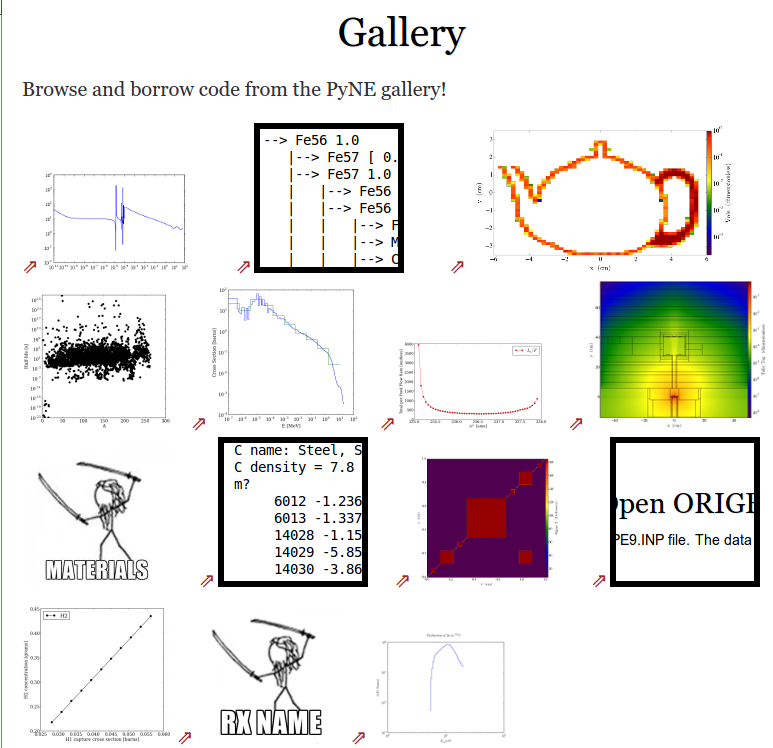
\includegraphics[height=2.75in,clip]{Gallery}
    \end{figure}
 	\end{center}

\end{frame}

%%%%%%%%%%%%%%%%%%%%%%%%%%%%%%%%%%%%%%%%%%%%%%%%%%%%%%
%%%%%%%%%%%%%%%%%%%%%%%%%%%%%%%%%%%%%%%%%%%%%%%%%%%%%%
\section{Current initiatives}
\begin{frame}{What are we Working on Now?}

    The biggest push: \textcolor{dgreen}{V\&V} $\rightarrow$ methodically making PyNE compliant 
    with the QA standards we've ratified, which are based on the ASME NQA-1 standards
    \cite{pyne_vnv}

    \vspace*{1 em}
    Many other items (large and small) in our ``ticket" list
    
    \begin{center}
 	\begin{figure}
 	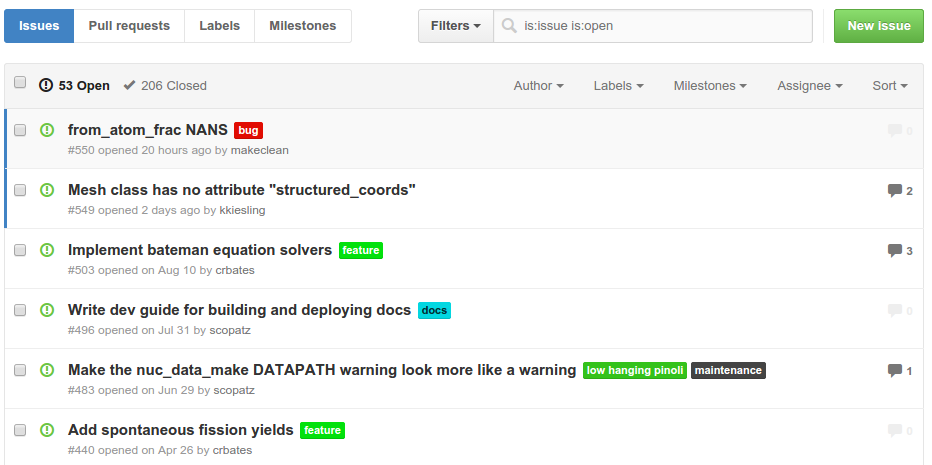
\includegraphics[height=1.75in,clip]{PyNE-tickets}
    \end{figure}
 	\end{center}
    
\end{frame}

%------------------------------------------------------
\begin{frame}{Verification and Validation}

    \textbf{Verification}: Have we built the software correctly?\\
    \textbf{Validation}: Have we built the correct software?
    
    \vspace*{1 em}
    Strategies employed by PyNE:
   
    \begin{itemize}
    \item Version control
    \item Formal review process
    \item Documentation: theory manual, user's guide, developer's guide, API, 
    ticket system
    \item Test suite
    \item Continuous Integration
    \end{itemize}

\end{frame}

%%%%%%%%%%%%%%%%%%%%%%%%%%%%%%%%%%%%%%%%%%%%%%%%%%%%%%
%%%%%%%%%%%%%%%%%%%%%%%%%%%%%%%%%%%%%%%%%%%%%%%%%%%%%%
\section{PyNE as a research tool}  
\begin{frame}{PyNE as a research tool}

    \textbf{Insight}: PyNE lets us access the physics, have real materials, 
    add mesh, and handle many details easily...
    
    	\pause
    \vspace{2 em}
    \textbf{Idea}: perfect environment for investigating numerical methods that 
    are impacted by materials, mesh, etc. 
    
    	\pause
    \vspace{2 em}
    \textbf{My Plan:} Plug-And-Play Solver Research Environment
    
\end{frame}

%------------------------------------------------------
\begin{frame}{What Are We Sovling?}

    I study how to solve the steady state, neutral particle Boltzmann transport equation
    more efficiently:
    %   
    \begin{align}
    [\vOmega \cdot \nabla + \Macro(\vec{r}, E)] &\psi(\vec{r}, \vOmega, E)  =  + q(\vec{r}, \vOmega, E) \nonumber\\
     &\int_0^{\infty} dE' \int_{4\pi} d\vOmega' \:\Macro_{s}(\vec{r}, E' \to E,
     \vOmega' \cdot \vOmega) \psi(\vec{r}, \vOmega', E') \nonumber
    \end{align}

    Discretize, then convert to operator form:
    \begin{align}
    \mathbf{L} \psi &= \mathbf{MS}\phi + \mathbf{Q} \nonumber\\
    \phi &= \mathbf{D}\psi \nonumber \\
    \underbrace{(\ve{I} - \ve{DL}^{-1}\ve{MS})}_{\mathbf{A}}\phi &= Q\nonumber
    \end{align}
    
    Properties of the matrix govern solution behavior
    
\end{frame}

%------------------------------------------------------
\begin{frame}{Discretizion Has an Impact}

    \begin{columns}
    \begin{column}{0.45\textwidth}
        \begin{center}
 	    \begin{figure}
 	    \includegraphics[height=1.75in,clip]{../figs/spatial-discretiztation2}
        \end{figure}
 	    \end{center}
  	\end{column}
   	%
 	\begin{column}{0.5\textwidth}
        There are many ways to \textcolor{dgreen}{discretize} the six dimensions of 
        phase space
        \begin{itemize}
        \item Spatial discretization methods
        \item Angular quadratures
        \item Energy group structures
        \end{itemize}
    
        \vspace*{1 em}
        \textcolor{dgreen}{Discretization} schemes and resolution choices can impact 
        numerical properites and/or solution strategies
  	\end{column}
	\end{columns}
 
\end{frame}

%------------------------------------------------------
\begin{frame}{So Does Physics}

    The physics of any specific problem also has a large impact on the
    problem's properties and solution strategies
    
    \begin{columns}
    \begin{column}{0.45\textwidth}
 	   \begin{center}
 	   \begin{figure}
 	   \includegraphics[height=1.75in,clip]{../figs/Fe-D2O-C}
 	   \caption{Iron-D2O-Graphite block energy S matrix; Evans et al.}
       \end{figure}
 	   \end{center}
  	\end{column}
   	%
 	\begin{column}{0.45\textwidth}
 	   \begin{center}
 	   \begin{figure}
 	   \includegraphics[height=1.75in,clip]{../figs/Fe-D2O-C-space-energy}
 	   \caption{Iron-D2O-Graphite energy-space-angle S matrix; Evans et al.}
       \end{figure}
 	   \end{center}
  	\end{column}
	\end{columns}
       
\end{frame}

%------------------------------------------------------
\begin{frame}{Properties Affect Solver Choice}

    \begin{columns}
    \begin{column}{0.45\textwidth}
        There are many ways to \textcolor{dgreen}{solve} this problem
        \begin{itemize}
        \item Inner iteration methods
        \item Outer iteration methods
        \item Eigenvalue iteration methods
        \item Preconditioners
        \end{itemize}
    
        \textcolor{dgreen}{Solution} method choices result in different
        behaviors for different systems
  	\end{column}
   	%
 	\begin{column}{0.45\textwidth}
 	   \begin{center}
 	   \begin{figure}
 	   \includegraphics[height=2.75in,clip]{solverLayers}
       \end{figure}
 	   \end{center}
  	\end{column}
	\end{columns}
	
\end{frame}
% All of the discretization choices and all of the solution stratgies create a complex set of choices

%------------------------------------------------------
\begin{frame}{Plug-And-Play Research Environment}

    Make collections of \textcolor{dgreen}{interchangeable pieces} for each component
    needed to construct a transport solver
    
    \vspace*{1em}
    Researchers can then 
    \begin{itemize}
    \item \textcolor{dgreen}{Assemble} a transport solver to fit their needs
    \item \textcolor{dgreen}{Add} their own new methods and investigate how 
    they interact with different solver combinations
    \end{itemize}

    \vspace*{1em}
    Implementing this in PyNE provides access to 
    \begin{itemize}
    \item PyNE's \textcolor{dgreen}{resources} such as nuclear data, materials, 
    and mesh tools  
    \item A flexible and robust \textcolor{dgreen}{development environment} 
    \item A well-managed \textcolor{dgreen}{API}
    \end{itemize}

\end{frame}

%------------------------------------------------------
\begin{frame}{Current Status}

    A collection of 3D spatial solver choices are available

    \renewcommand\windowpagestuff{%
    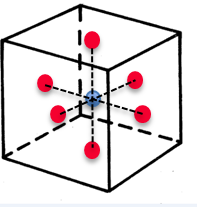
\includegraphics[height=1in,clip]{../figs/spatial-cell}
    \raggedright}
    \opencutright
    \vfill
    \begin{cutout}{9}{0.7\textwidth}{0pt}{2}
    \begin{itemize}
    \item DGFEM: Lagrange, Complete; Simple Corner Balance; AHOTN; Linear Nodal;
     Linear-Linear; Diamond Difference type
    
    \item Originally written in Fortran (Sebastian Schunert and Yousry Azmy,
    \textcolor{cardinal}{NC State})

    \hspace*{2 em}[PyNE's first Fortran!]
    
    \item Wrapped with f2py (Josh Howland, \textcolor{byellow}{Berkeley})
    \item Accessible via PyNE interface   
    \item Examples, tests, documentation
    \end{itemize}
    \end{cutout}
    
\end{frame}

%------------------------------------------------------
\begin{frame}{Next Steps}

    \begin{columns}
    \begin{column}{0.5\textwidth}
        \begin{itemize}
        \item Establish plug-in framework
        \item Retool spatial solvers as necessary
        \item Add quadrature sets
        \item Implement/access the most common solvers
        \item Add preconditioners
        \end{itemize}
  	\end{column}
   	%
 	\begin{column}{0.4\textwidth}
        \begin{center}
 	    \begin{figure}
 	    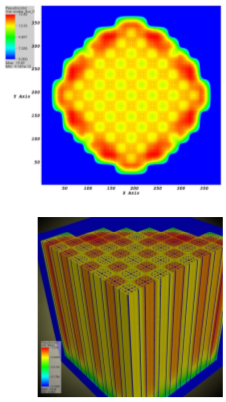
\includegraphics[height=2in,clip]{../figs/PWR-maps}
 	    \caption{PWR Flux Maps from Denovo; Joubert et al.}
        \end{figure}
 	    \end{center}
  	\end{column}
	\end{columns}
    
\end{frame}

%%%%%%%%%%%%%%%%%%%%%%%%%%%%%%%%%%%%%%%%%%%%%%%%%%%%%%
%%%%%%%%%%%%%%%%%%%%%%%%%%%%%%%%%%%%%%%%%%%%%%%%%%%%%%
\section{Get involved!}
\begin{frame}{Why Would I Get Involved?}

    As a \textcolor{dgreen}{user} 
    \begin{itemize}
    \item You could do your work or research with PyNE
    \item Even if you have your own software that looks and behaves similarly to some aspects of PyNE, using PyNE will mean that you no longer have to develop AND maintain that functionality
    \end{itemize}        

    \vspace*{1 em}
    As a \textcolor{dgreen}{developer} 
    \begin{itemize}
    \item You should be selfish
    \item Contribute to PyNE in ways that support the work that you are doing
    \item If a feature you want is not in PyNE right now, chances are that other 
    people want to see that feature too
    \item This will help your future self as much as future other people
    \end{itemize}    

\end{frame}

%------------------------------------------------------
\begin{frame}{How Can I Get Involved?}

    \textcolor{dgreen}{Contact PyNE}
    \begin{itemize}
    \item Website: \href{http://pyne.io/}{\texttt{http://pyne.io/}}
    
    \item User's Mailing List: \href{pyne-users@googlegroups.com}
    {\texttt{pyne-users@googlegroups.com}}
    
    \item Developer's List: \href{pyne-dev@googlegroups.com}
    {\texttt{pyne-dev@googlegroups.com}}
    
    \item GitHub: \href{https://github.com/pyne/pyne}
    {\texttt{https://github.com/pyne/pyne}}
    
    \item Tutorial: \href{http://pyne.io/tutorial/index.html}
    {\texttt{http://pyne.io/tutorial/index.html}}
    \end{itemize}
    
    \vspace*{2 em}
    \textcolor{dgreen}{What goes into PyNE?}

    Anything that is not export controllable, proprietary, 
    or under HIPPA restrictions!  (If you have questions, ask)
  
\end{frame}


%%%%%%%%%%%%%%%%%%%%%%%%%%%%%%%%%%%%%%%%%%%%%%%%%%%%%%
%%%%%%%%%%%%%%%%%%%%%%%%%%%%%%%%%%%%%%%%%%%%%%%%%%%%%%
\section*{}
\begin{frame}[fragile]{Questions?}

    \begin{center}
    \includegraphics[height=3in,clip]{../questions-comic}  
    \end{center}
  
\end{frame}

% --------------------------------------------------------------
\begin{frame}[fragile]{PyNE In the Literature}

    \begin{itemize}
    \item Intro: "PyNE: Python For Nuclear Engineering" \cite{pyne_intro}
    \item Progress reports: \cite{scopatz_pyne}, \cite{pyne_progress}
    \item In research: \cite{Biondo2014}, \cite{MarquezDamian2014280}, \cite{Scopatz2013a}
    \item V\&V: "Quality Assurance within the PyNE Open Source \\Toolkit" \cite{pyne_vnv}
    \item Poster at SciPy: \cite{scipy}
    \end{itemize}
  
\end{frame}
% --------------------------------------------------------------
\begin{frame}[allowframebreaks]{References}
	\bibliographystyle{unsrt}
	\bibliography{2014-10-norcal-ans-pyne.bib}
\end{frame}

\end{document}
